\documentclass[USenglish]{article}

%\usepackage[utf8]{inputenc}%(only for the pdftex engine)
\RequirePackage[no-math]{fontspec}[2017/03/31]%(only for the luatex or the xetex engine)
\usepackage[small]{dgruyter}

\usepackage{natbib}
\bibliographystyle{apalike}

\usepackage{microtype}

\begin{document}

  \articletype{Research Article}

  \author*[1]{C.J.(Chaojie) Duan}
  %\author[2]{...}
  %\author[1]{...} 
  %\runningauthor{Duan}
  \affil[1]{Dulun Consulting Group, research@dulun.com}
  %\affil[2]{...}
  \title{Latent vs. Observable Home-Field Advantage in Professional Soccer}
  \runningtitle{Bayesian Hierarchical Analysis}
  \subtitle{A Multilevel Bayesian Operationalization}
  \abstract{Home Field Advantage (HFA) was traditionally defined in terms of the winning percentage of home games at the team level. In this article, we present a hierarchical model of HFA, spanning from the top sport level to the middle league level and all the way to lowest club level. Using scoring performance data from ESPN FC, we fit a Bayesian multilevel nested model to the parameters in the hierarchical model of HFA, allowing information obtained from the season level to inform the inferences about scoring capabilities at the upper team, league, and sport levels. On the one hand, our analysis reveals that much of HFA is attributed to the nature of the sport of interest. League level source of HFA , on the other hand, can be safely ignored. While only a handful of teams out of 98 in top 5 European leagues enjoy statistically significant HFA, we found absolutely no teams suffer from home disadvantage.}
  \keywords{European Professional Soccer Leagues, Latent Home Field Advantage, Poisson generative process, Stan}
  %\classification[PACS]{...}
  %\communicated{...}
  %\dedication{...}
  \received{4/24/2018}
  %\accepted{...}
  \journalname{Journal of Quantitative Analysis in Sports}
  %\journalyear{...}
  %\journalvolume{..}
  %\journalissue{..}
  \startpage{1}
  %\aop
  %\DOI{...}
\maketitle

\section{Introduction} 

 

In professional team sports, the term home field advantage (HFA) – also called home advantage, home ground or home court advantage, defender's advantage, home-ice advantage – describes the benefit that the home team is believed to gain over the visiting opponent. Its scientific definition is ``the consistent finding that home teams in sport competition win over 50\% of the games played under a balanced home and away schedule'' \citep[p. 13]{Courneya1992}.
Due to the existence of HFA, many vital games, such as playoff or elimination matches, in major professional sports have special rules for determining which match is played at which place.  As shown in Figure \ref{fig11}, the combined revenue of the Big Five European soccer leagues (English Premier League, Spanish La Liga, French Ligue 1, Bundesliga, Italian Serie A) more than doubled to 15 billion euros in 10 years from 2006/07 to 2016/17. The financial implications might partially explain UEFA's (the Union of European Football Associations) decision that a second leg of any Champions League knock-off series is favorable to playing away with the the scores still in balance after the first leg competition \citep{atkins2013}.

%----------------------
\begin{figure}[ht]
\caption{\textit{Revenue of the top European soccer leagues (Big Five*) from 2006/07 to 2016/17 (in billion euros)}}
\centering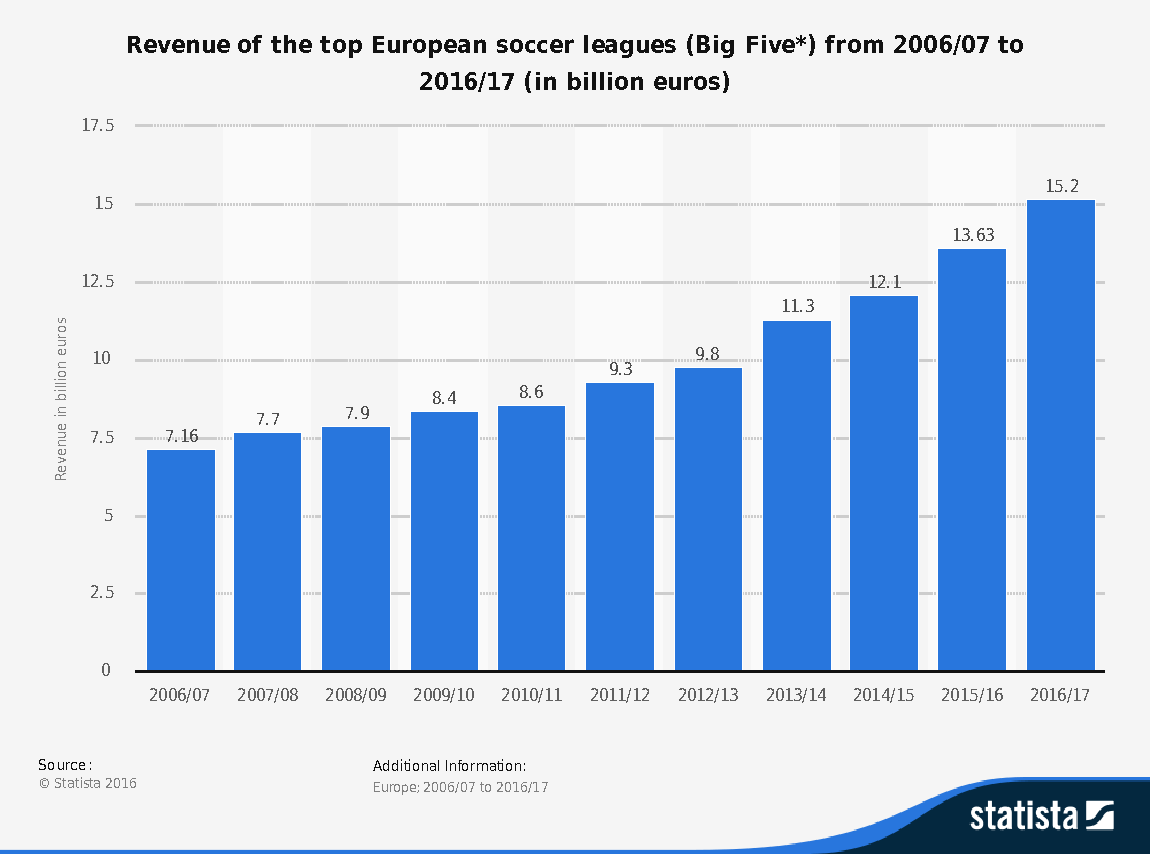
\includegraphics[width=0.8\textwidth]{HFA11.pdf}. 
\label{fig11}
\end{figure}
%------------------------

The existence of HWP (home winning percentage) -denominated HFA measure has been well documented for a variety of sports, even though the contributing factors are still being debated. In their book \textit{Scorecasting}, \cite{moskowitz2012scorecasting} compiled the HWPs in all the major sports with some datasets going back as further as 1903 for MLB and 1966 for NFL. MLS figures date back to only 2002, but show the strongest evidence of HWP of 69.1\%. MLB figures, on the other hand, yield the lowest HWP of only 53.9\%. This disparity raises an important high-profile question: ``Are all sports created equal in terms of HFA?''. A subsequent but related question is ``Is HFA primarily determined by the sport being played or teams who play the sport?''. Answering such questions demands a completely new way of conceptualizing HFA and signals a major departure from the reigning framework proposed by \cite{Courneya1992}, which hinges on game being the unit of analysis.  
 
A second motivator for this study is related to the treatment of sports data in general, and scoring in soccer matches in particular. HWP based measures tend to upstage and upgrade the originally discrete count-based outcome to continuous type, while ignoring the underlying data generating process. To complicate matters further, consider the two extreme cases of all winning and losing regular season. The HWP and AWP(away winning percentage) are equal, taking values of either 1.o or 0.0. If we adopt HWP as the sole indicator of HFA, we go straightforward to absurd conclusions - the all winning club enjoys 100\% HFA and the zero-win team suffers from 100\% home field disadvantage.   

The current conceptualization and operationalization of HFA prompt us to take an alternative route in search of the true latent HFA underlying the numbers in record books. Specifically, we seek in this paper to achieve the following goals: 

\begin{enumerate}
\item  Propose a fresh new vertical hierarchical model of HFA, complementing the existing horizontal framework.
\item Highlight the different generative process underlying most sports performance metrics and suggest corresponding approaches for analysis.
\item Reveal sources of HFA simultaneously at sport, league, team levels.
\item Presenting a new way of measuring latent HFA via contrasting the same performance metric at home and away venues. 
\end{enumerate}

The remainder of the paper is structured as follows: In the section immediately after this opening introduction, we review relevant literature and assemble existing knowledge for the development of our unique hierarchical view of HFA. 
In the section of \textit{Definition of the Hierarchical Model}, we construct a full HFA-specific probabilistic model, which is mainly a joint probability distribution for all observed and latent quantities in a problem, consistent with domain knowledge and the data collection process.
In the next section of \textit{Data and Results}, we compute and display the posterior distributions of the unobserved model parameters, given the observed data collected from ESPN FC website. Also in the same section, we evaluate the fit of the hierarchical model in the context of model comparison and posterior predictive checking. We close our paper with limitations and directions for future HFA research.
%\end{enumerate}
 
\section{Review of Literature} 

The UEFA oversees 55 European country-level member associations (such as the English Football Association- EFA), which in turn oversees all professional football leagues within their respective jurisdictions. Figure \ref{fig21} provides a rough sketch of the organizational structure of professional football in Europe, with an emphasis on the elite Top 5. According to UEFA's mission statement,``UEFA's core mission is to promote, protect and develop European football at every level of the game, to promote the principles of unity and solidarity, and to deal with all questions relating to European football ... UEFA is an association of associations based on representative democracy, and is the governing body of European football. Football is the priority in everything that we do''.
In conjunction with its 55 member associations, the union strives to nurture and promote the European refereeing sector  and ensure that newcomers to the UEFA list are given the proper training for their duties.

The speed and movement in top-level football competition, allied to the intense scrutiny of media on the actions on the field, means that officiating crews must be well-prepared, possess the tactical acumen, the mental strength to withstand pressure and the ability to take split-second decisions with confidence and consistency. Such split-second decisions made under severe pressure from home crowds have been proved to show systematic favoritism for the home squad   
both experimentally \citep{Nevill1999, Nevill2002} and in observational settings \citep{Nevill1996, DOHMEN2008}.
%------------------------------------------------
\begin{figure}
\caption{The Hierarchical Structure of Professional Soccer }
{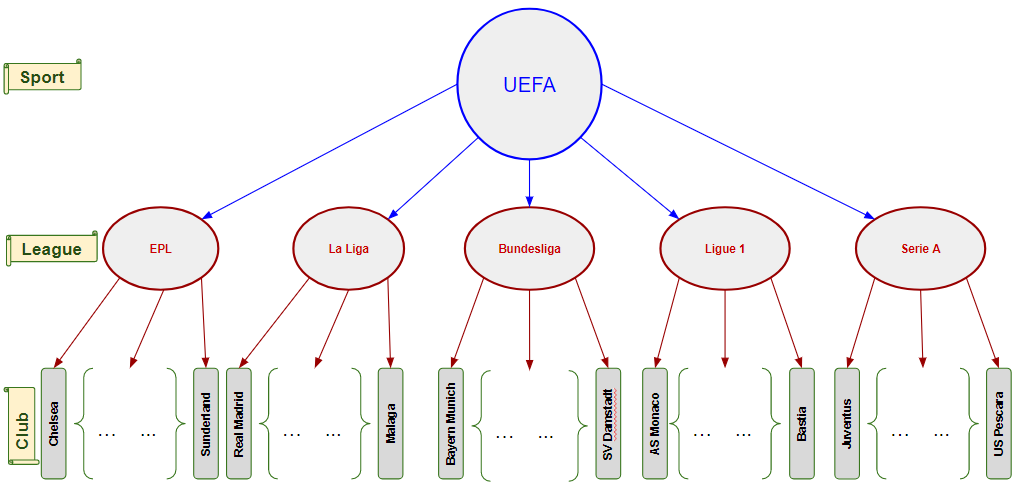
\includegraphics[width=1.0\linewidth]{HFA_22}}
\label{fig21}
\end{figure} 
%------------------------------------------------ 

Following the episode of hooligan-induced riot on Feb. 2, 2007, the Italian authorities forced soccer clubs with deficient security standards at their home stadiums to play their home games with no spectators. The ruling inadvertently created a sizable and scarece sample of 21 professional soccer games played before empty bleachers. \cite{Pettersson-Lidbom2010} seized on this historical opportunity and contrasted the performance metrics of both referees and players by looking at the matches played by the same team and officiated by the same referee crew. They found convincing evidence for the effect of spectators on referees, manifested in the 70\% (26\%) drop for red (yellow) cards issued favoring the home team. On the other hand, the players did not seem to play any differently whether the yelling crowds were present or absent. 

With game as the anchoring unit of analysis, \cite{Courneya1992} developed a conceptual framework along the timeline axis of a typical soccer game. For simplicity of reference and purpose of contrasting, we designate their framework as the horizontal view of HFA (HVHFA). From left to right along the axis, HVHFA incorporates five major components: game site location, game location factors, psychological states, behavioral sates, and the final performance outcomes. At the end of their review, they pointed out that future research should be directed at factors causing HFA rather than the verification of its existence. After taking stock of decades' HFA research findings suffused with equivocality, \cite{Carron2005} surprisingly revised the original HVHFA with the deletion of ``officials'' and the inclusion of ``psychological states''. The rationale behind their removal of officiating factors is rather methodological inconvenience. Unlike spectators, players and coaches, referees and umpires can't be easily assigned to either hosting or visiting status for each game they officiated. 


\cite{Pollard1986} discovered that the extent of HFA in English soccer has remained relatively consistent since the formation of the English Football League in 1888. The time-invariant tendency, coupled with the largest betrayed effect, makes professional soccer an excellent venue for studying HFA at a more aggregate level beyond individual matches and even seasons. 

 

As \cite{Boyko2007} pointed out, traditional frequentist statistical approaches don't address whether referees or players alone or combined channel crowd effects to impart on final match outcome. Bayesian inferential approach separates itself from its frequentist counterpart due to its emphasis on modeling all forms of uncertainty rather than providing point estimates. Regardless of the inferential approaches taken, one major goal of statistical analysis is model selection among a set of competing models that were assumed to have generated the observed data. With the aid of posterior predictive checking \citep{Gelman1996}, researchers can assess the fitness of competing models with realized discrepancies between the actual and replicated data points. 

With the rare exception of \cite{Gajewski2006} and \cite{Glickman1998, Glickman2005}, Bayesian statistical approach has not been widely adopted in the analysis of HFA. One unique feature of the \cite{Gajewski2006} study is that they model longitudinal data across seasons while utilizing a unique HFA parameter dedicated to each team involved in the investigation. One problem common to these Bayesian studies is that they directly model the match-based goal differentials between the hosting and visiting teams. Such estimates based on score differentials of individual matches are effectually  blending home team's HFA and visitors' guest field disadvantage. Thus, we sense an urgent need to break down HFA into sub-components, which we can pinpoint to their originating sources.    

The subject and methodology-matter motivations for this research lie in the decomposition of home field advantage in a multilevel format that naturally reflects the structure of professional soccer competition. With the help of Bayesian nested modeling, we shall demonstrate next how easily we can alter the structural complexity of the main candidate model with just a few lines of code.

\section{Definition of the Hierarchical Model} 

The essence of Bayesian inference is fitting a probability model to a dataset and generating probability distributions on the parameters encapsulated by the model \citep{Gelman2014}.

%------------------------------------------------
\begin{figure}
\caption{The Hierarchical Model of Home Field Advantage }
{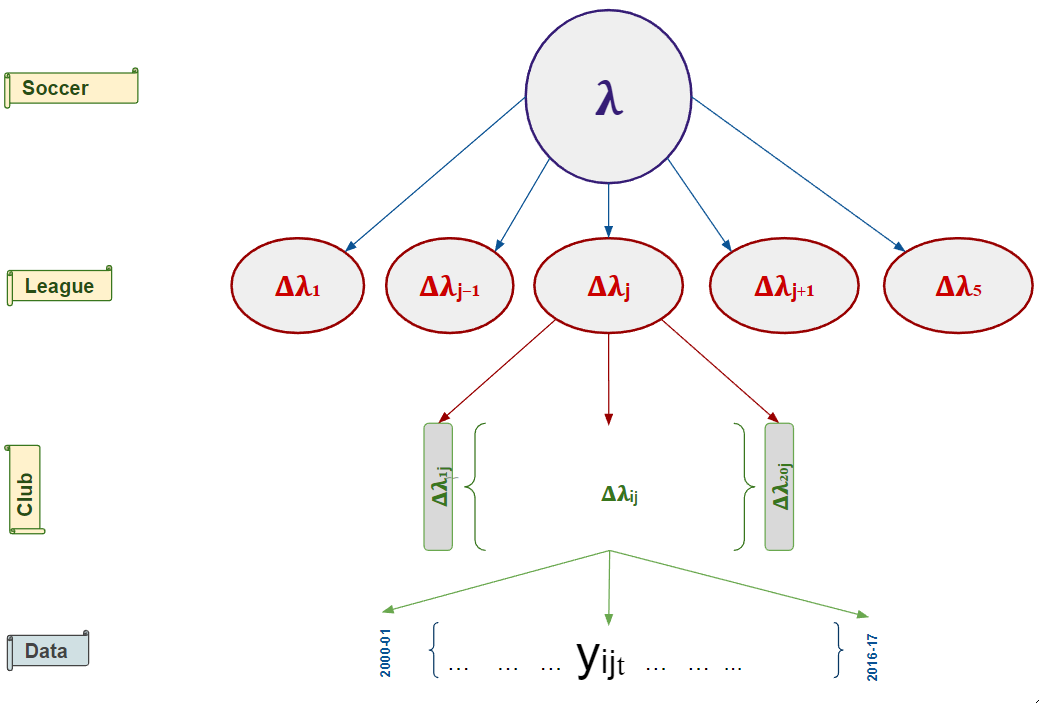
\includegraphics[width=1.0\linewidth]{HFA_33}}
\label{fig33}
\end{figure} 
%------------------------------------------------ 

 
For our project, the data set contains the season (s) -level best home and away scoring numbers ($y^H_{ijs}$ and   $y^A_{ijs}$ respectively) of each club i in each j of the Top 5 leagues. As shown in figure \ref{fig33}, our hierarchical model reflects the organizational structure of professional soccer shown in figure \ref{fig21}. We treat the generative processes of $y^H_{ijs}$ and $y^A_{ijs}$ as similar but independently governed by their own respective parameters. At the measurement level, we encode $y^H_{ijs}$ and $y^A_{ijs}$ into corresponding latent scoring rate $\lambda^H_{ij}$ and $\lambda^A_{ij}$ with Poisson distribution, which is a commonly accepted distributional model for sports count data \citep{Miller2015}:

Because team i is nested within league j, we can decompose the latent $\lambda_{ij}$ into $\Delta_{ij}+\lambda_j$ and thus acquire inference about league level latent scoring rate $\lambda_j$. By the same token, we can drill $\lambda_j$ down into $\Delta_{j}+\lambda$ and estimate sport level latent scoring rate of $\lambda$. In the final step, we take the differentials between the three matched pairs of home-away scoring rates and express the hierarchical model of HFA formally as the set of equations consisting of (1), (2),(3), and (4). 

\begin{equation}
\begin{cases}
y^H_{ijs} \sim Poisson(\lambda^H_{ij})\\
y^A_{ijs} \sim Poisson(\lambda^A_{ij})
\end{cases}
\end{equation}

\begin{equation}
\begin{cases}
\delta_{ij} = \lambda^H_{ij} - \lambda^A_{ij}\\  
\Delta^H_{ij}, \Delta^A_{ij}  \sim N(0, \sigma^2_c)\\  
\sigma_c \sim cauchy(0,2)
\end{cases}
\end{equation} 

\begin{equation}
\begin{cases}
\delta_{j} = \lambda^H_{j} - \lambda^A_{j}\\  
\Delta^H_{j}, \Delta^A_{j} \sim N(0, \sigma^2_l)\\
\sigma_l \sim cauchy(0,2)
\end{cases}
\end{equation} 

\begin{equation}
\begin{cases}
\delta = \lambda^H - \lambda^A\\
\lambda^H, \lambda^A \sim cauchy(0, 10)
\end{cases}
\end{equation} 

As outlined in Figure \ref{fig33} and above equations, the total number of parameters included in the full model is 208, including 2 $\lambda$s at the top + 2 X 5 $\Delta$s at the league level + 2 X 98 team-level $\Delta$s. In addition, there are two hyper-parameters ($\sigma$) governing the distribution of league and team level parameters.

\section{Data and Results} 

For practical reasons, the Top 5 leagues serve as a convenient sample as performance data at season level are reliable and retrievable via internet.  On ESPN FC website, we find a pair of venue-delineating (home and away) goal scoring metrics used to characterize a professional soccer club's regular season. Below, we define those statistics using the 2015/16 La Liga season of Real Madrid C.F. as an example.

\begin{itemize}
\item Most Home Goals (as $y^H_{ijs}$) = maximum goals scored in a single match played at home. For the season 2015/2016, Real Madrid’s $y^H_{3,1,16}$ is 10. They beat Rayo Vallecano by 10-2 at Santiago Bernabéu Stadium on 12/20/2015.
\item Most Away Goals (as $y^A_{ijs}$) = maximum goals scored in a single away match. For the season 2015/2016, Real Madrid’s $y^A_{3,1,16}$ is 6. They defeated Espanyol 6-0 on 9/12/2015 at RCDE stadium.
\end{itemize}

Table \ref{tab1} provides the summary statistics of $y^H_{ijs}$ and $y^A_{ijs}$. Both averages and medians evince the existence of positive goal differential between maximum home and away goals. However, the MAG is more skewed than MHG in that the max. of MAG is actually greater than that of MHG. Deletion of such outliers is not an option in conducting sports analytics, because they are quintessential of the underlying exceptional performance by athletes. Fortunately, Bayesian statistics can accommodate such wide dispersion of data points with alternative distribution functions other than the commonly-applied Gaussian PDF (normal probability density function). 

%-----------------------
\begin{table}[ht]
\caption{Descriptive Statistics}
\centering
\begin{tabular}{cccccccc}
\starttabularbody
\hline 
 & Mean & Median & Std. Dev. & Min. & Max. & Skewness & Kurtosis\\
\hline
 MHG & 3.634 & 4 & 1.676 & 0 & 9 & 0.246 & 0.034 \\
\hline 
 MAG & 2.884 & 3 & 1.676 & 0 & 10 & 0.627 & 0.786 \\
\hline
\end{tabular}
\label{tab1}
%{Goal Scoring Metrics: Most Home \& Away Goals at the Season Level} 
\end{table}
%=====================================================

We fit our model with 4 chains of length 999 (with the first 1/3 for warmup) using the default sampler in Stan, the HMC variant of No-U-Turn Sampler (NUTS) \citep{Hoffman2014}.  

The sport and league level estimates of goal-scoring rate differential are shown in Figure \ref{fig31} as shift from the 0. The outer contour line depicts the 99.5\% uncertainty intervals, while the shaded area underneath covers the corresponding 95\% uncertainty intervals. The light bar in the middle represents the mean.

\begin{figure}
\caption{HFA Posterior Plot at Sport and League Levels}
\centering
{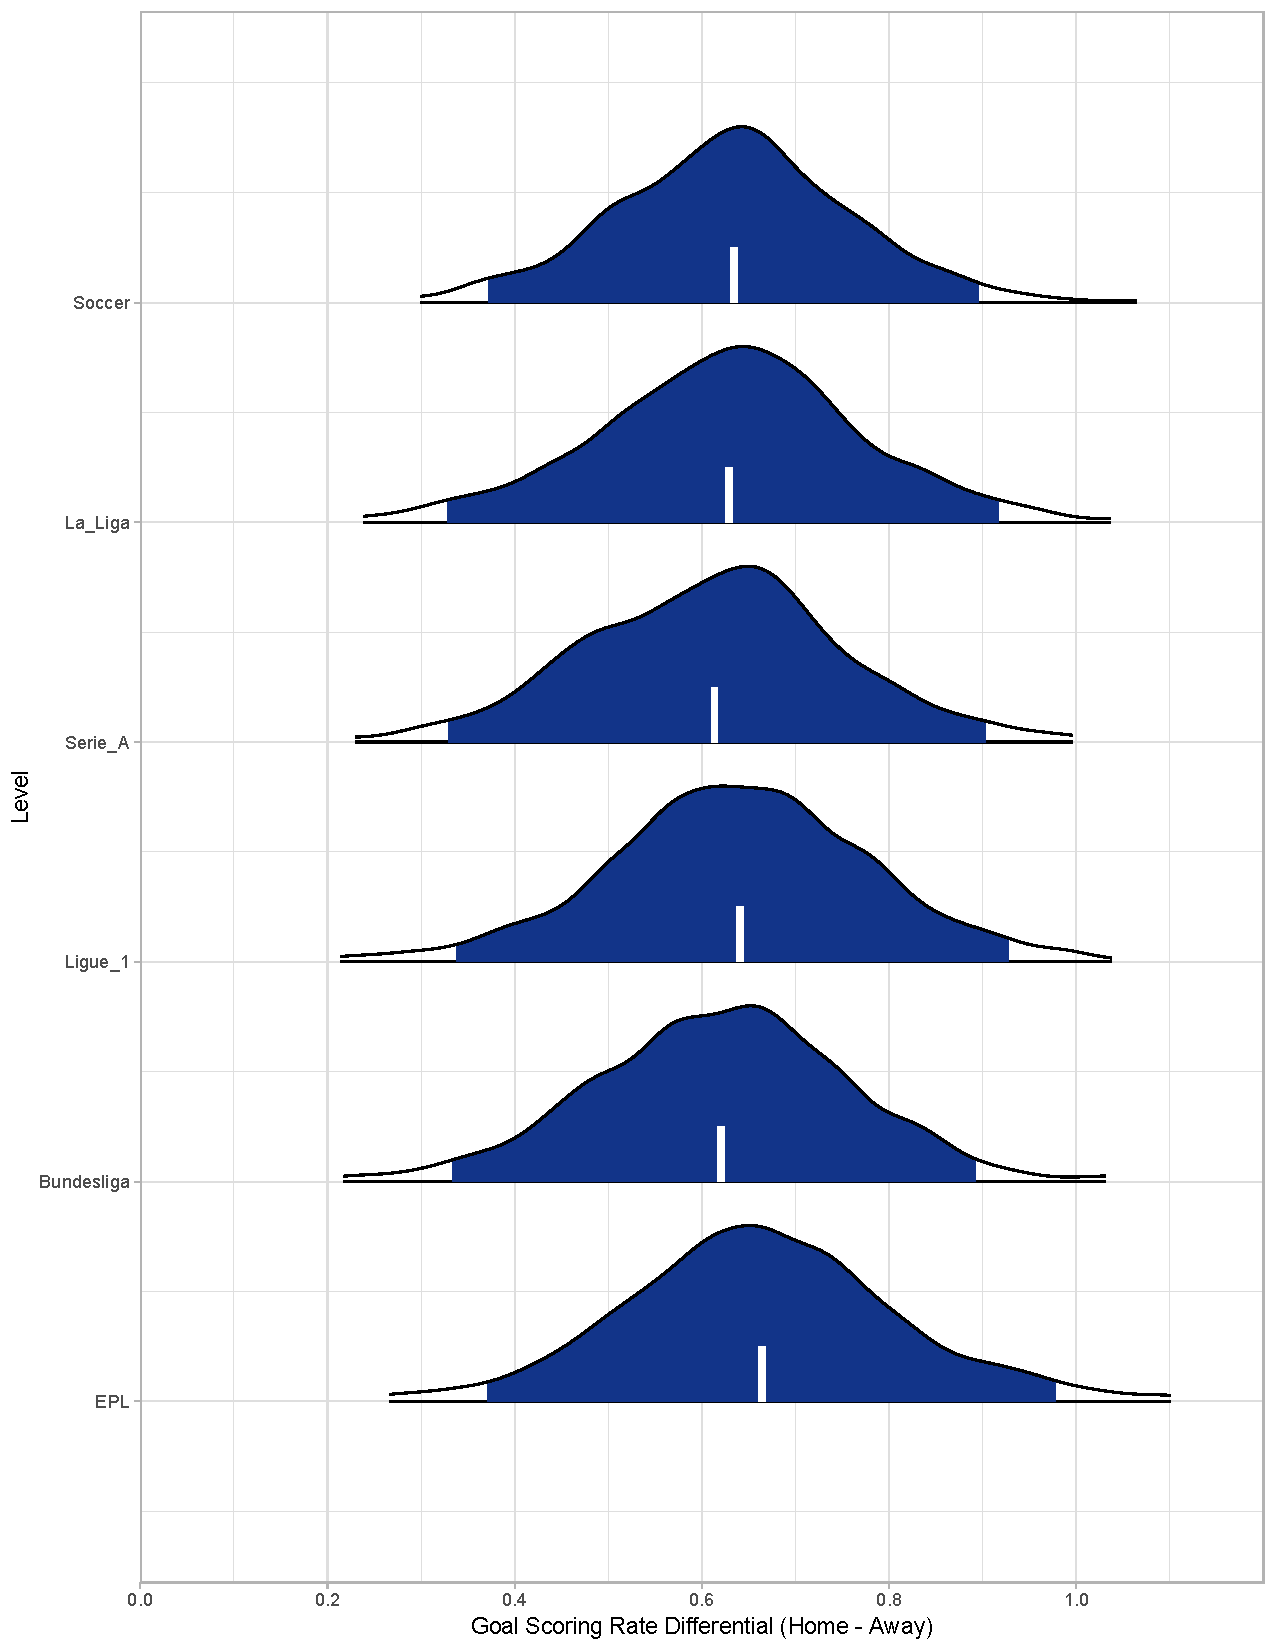
\includegraphics[width=1.00\linewidth]{HFA32.pdf}}
\label{fig31}
\end{figure}

In Figure \ref{fig31}, we observe absolutely strong (99.5\%) manifestation of HFA for the sport of soccer. The goal-scoring differentials are centered around 0.65 goals with comparable lengths of uncertainty intervals.  
It is also clear that the Top 5 leagues as a whole did not assert much influence on either location or shape of the parameters of interest at the league level. The English Premier League was able to slightly push the center close to 0.7 goals, which indicates EPL teams enjoy relatively stronger HFA.

\begin{figure}
\caption{Home Field Advantage Posterior Plot for La Liga Teams}
{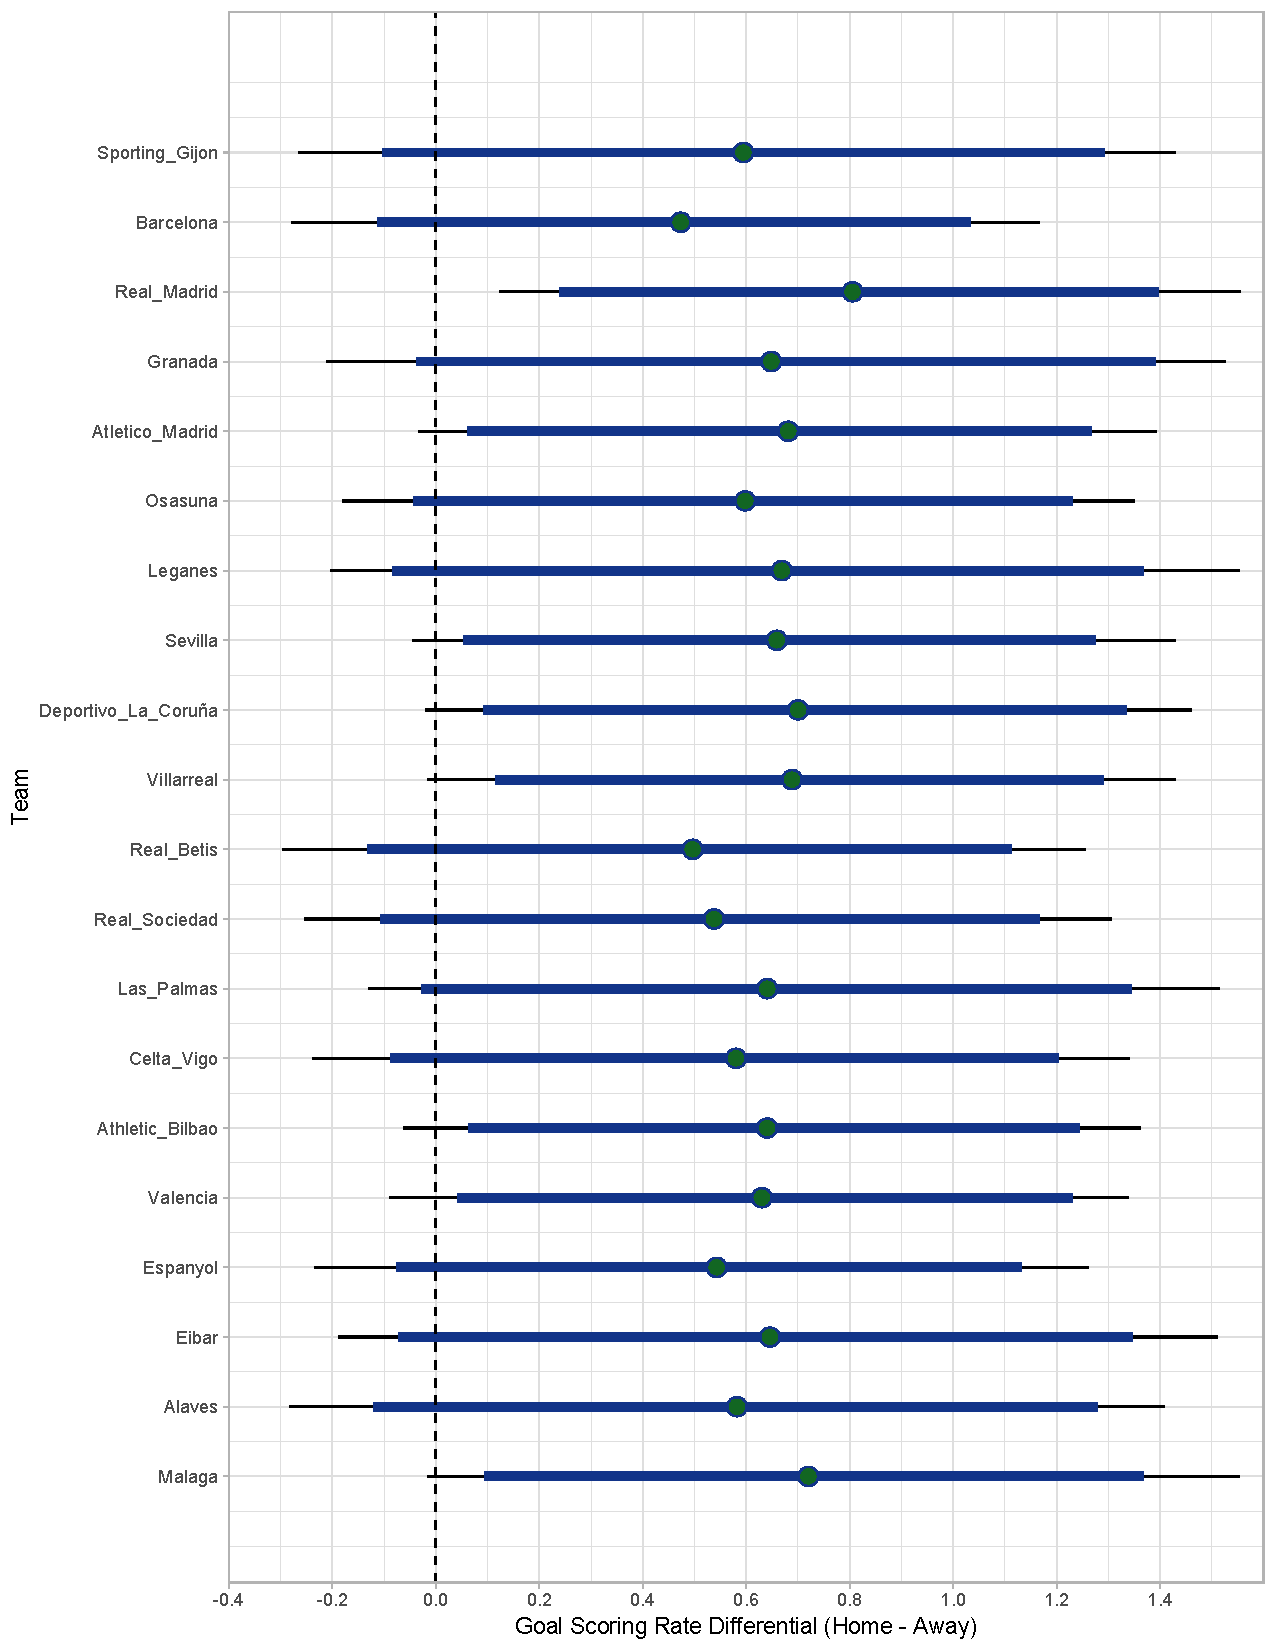
\includegraphics[width=0.90\linewidth]{HFA_La_Liga11.pdf}}
\label{fig32}
\end{figure}

To summarize team level estimates, we use the outer thin line and the inner thick line to represent the 95\% and 90\% uncertainty intervals respectively. The dot in the middle still represents the mean as before.


As shown in Figure \ref{fig32}, Real Madrid is the only club in La Liga enjoys strong HFA with the left tip of its 95\% uncertainty interval not crossing the dashed line of zero. Another 7 teams enjoy marginal HFA with the left tips of their 90\% uncertainty interval not crossing the dashed line of zero. It is noteworthy that the worst performer of the current 2016/17 season - Malaga - enjoys almost strong HFA.     

\begin{figure}
\caption{Home Field Advantage Posterior Plot for Serie A Teams}
{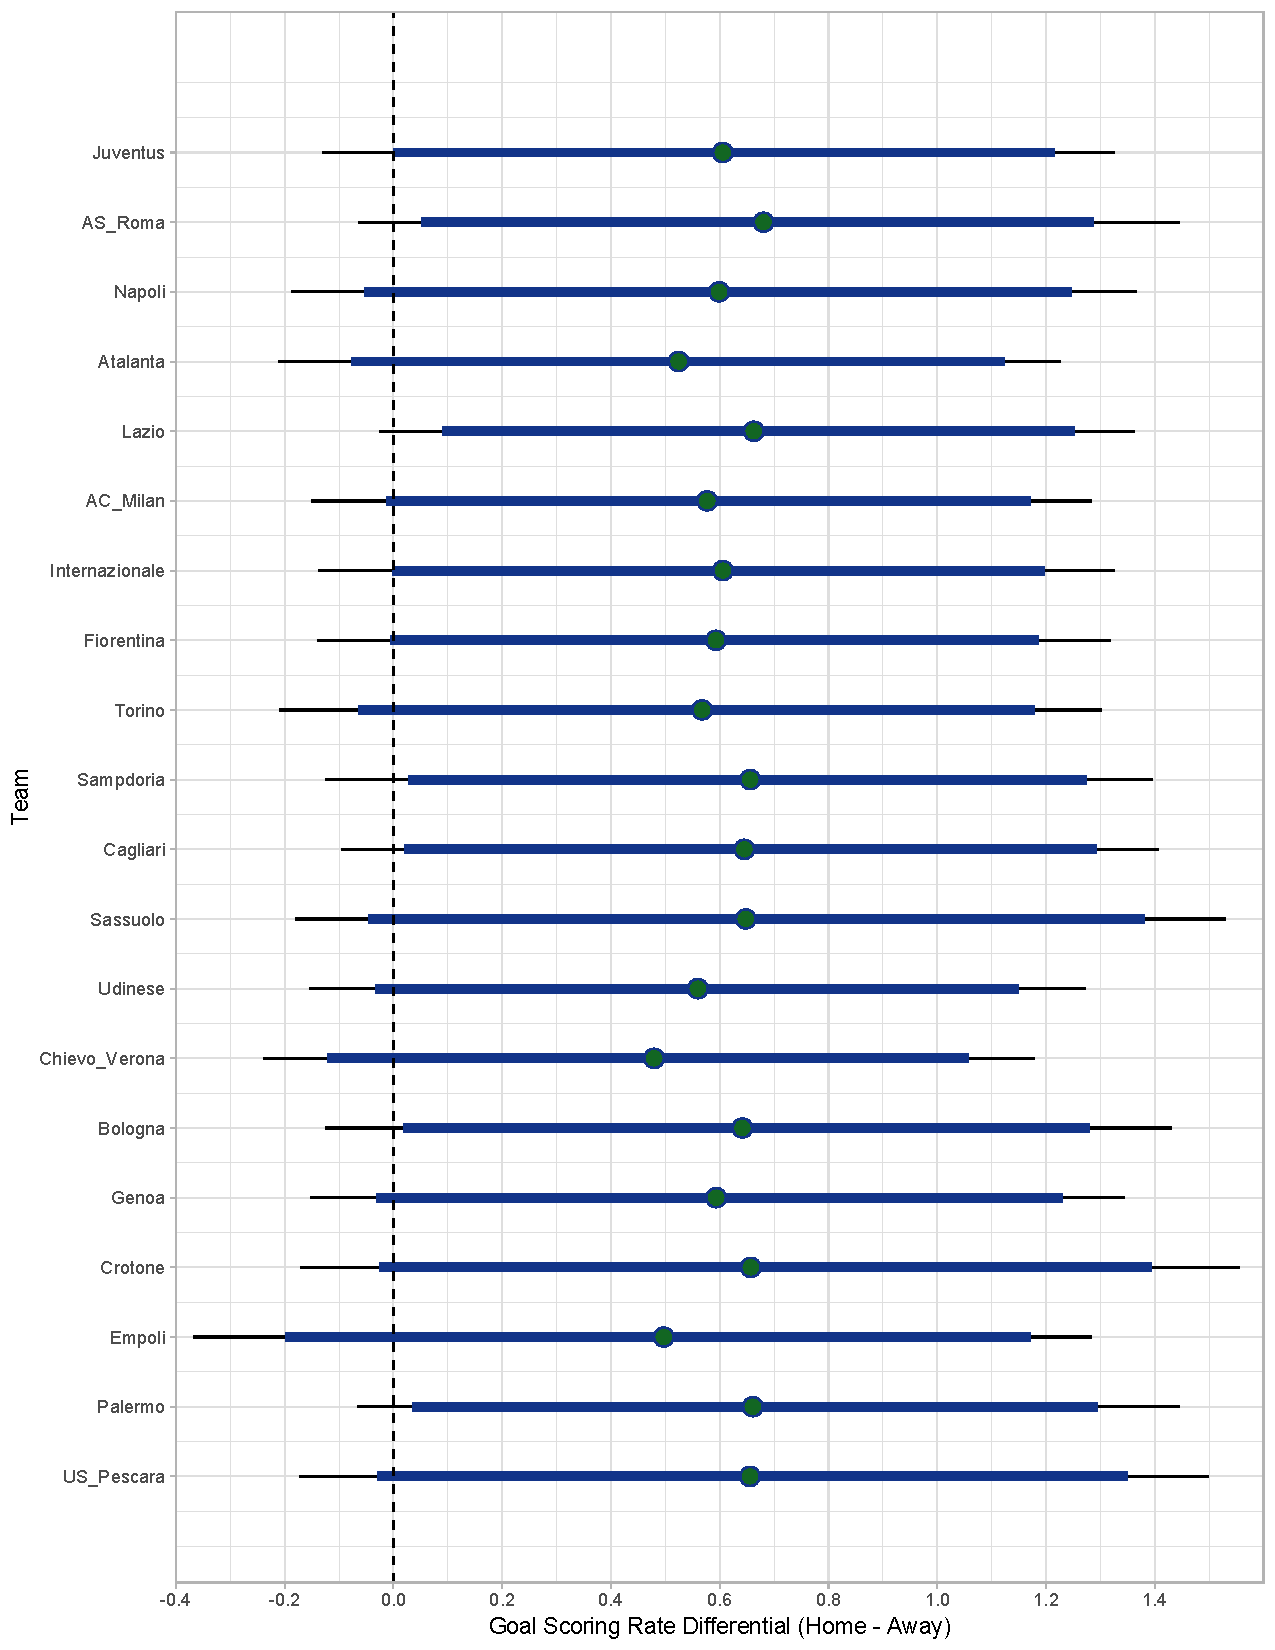
\includegraphics[width=0.90\linewidth]{HFA_Serie_A11.pdf}}
\label{fig4}
\end{figure}

For Serie A, Figure \ref{fig4} paints a different picture. Only a total of 6 out of 20 clubs exhibit marginal HFA. As displayed in Figure \ref{fig5}, the number of teams enjoying marginal HFA improved to 10 out of 20 for French Ligue 1. Still, no teams in Ligue 1 boast statistically significant HFA at the 95\% level. In Figure \ref{fig6}, Bundesliga demonstrates a similar pattern with only 9 teams in possession of marginal HFA.   

\begin{figure}
\caption{Home Field Advantage Posterior Plot for Ligue 1 Teams}
{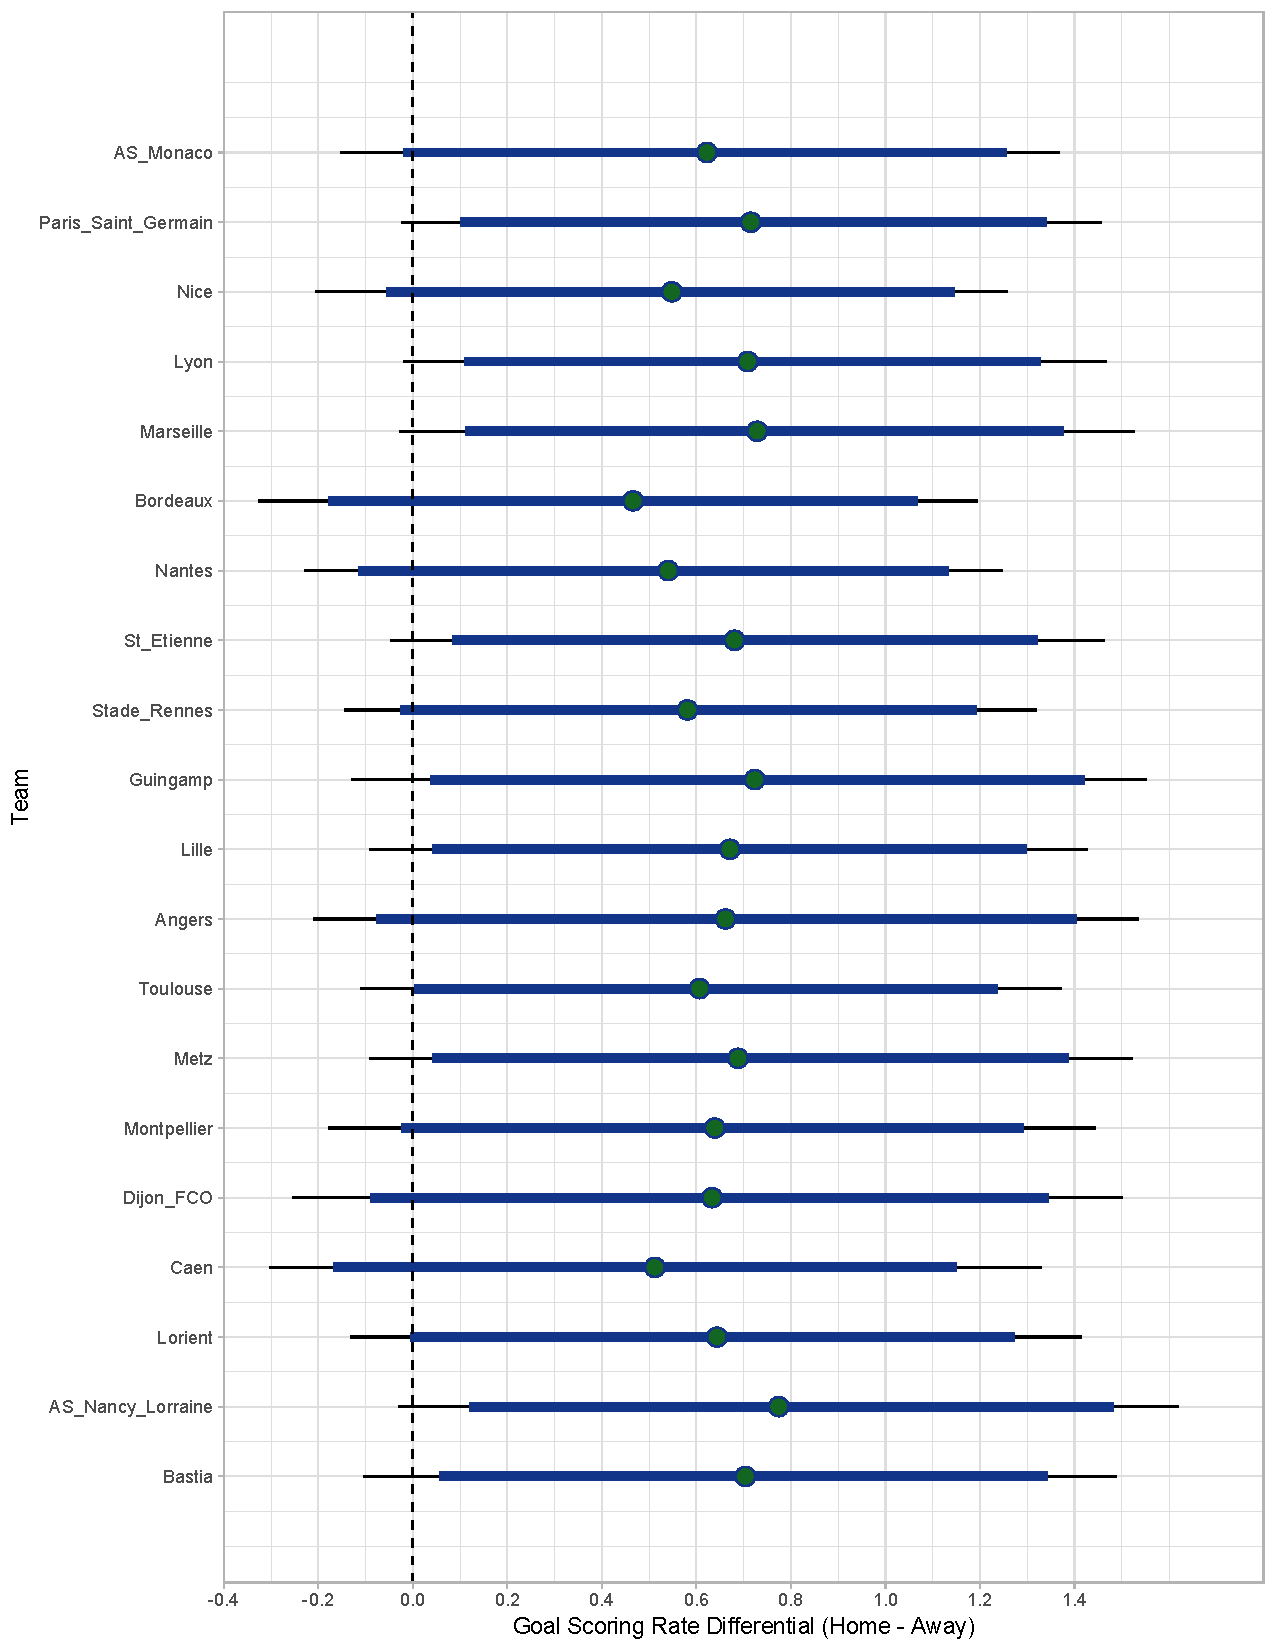
\includegraphics[width=0.90\linewidth]{HFA_Ligue111.pdf}}
\label{fig5}
\end{figure}

\begin{figure}
\caption{Home Field Advantage Posterior Plot for Bundesliga Teams}
{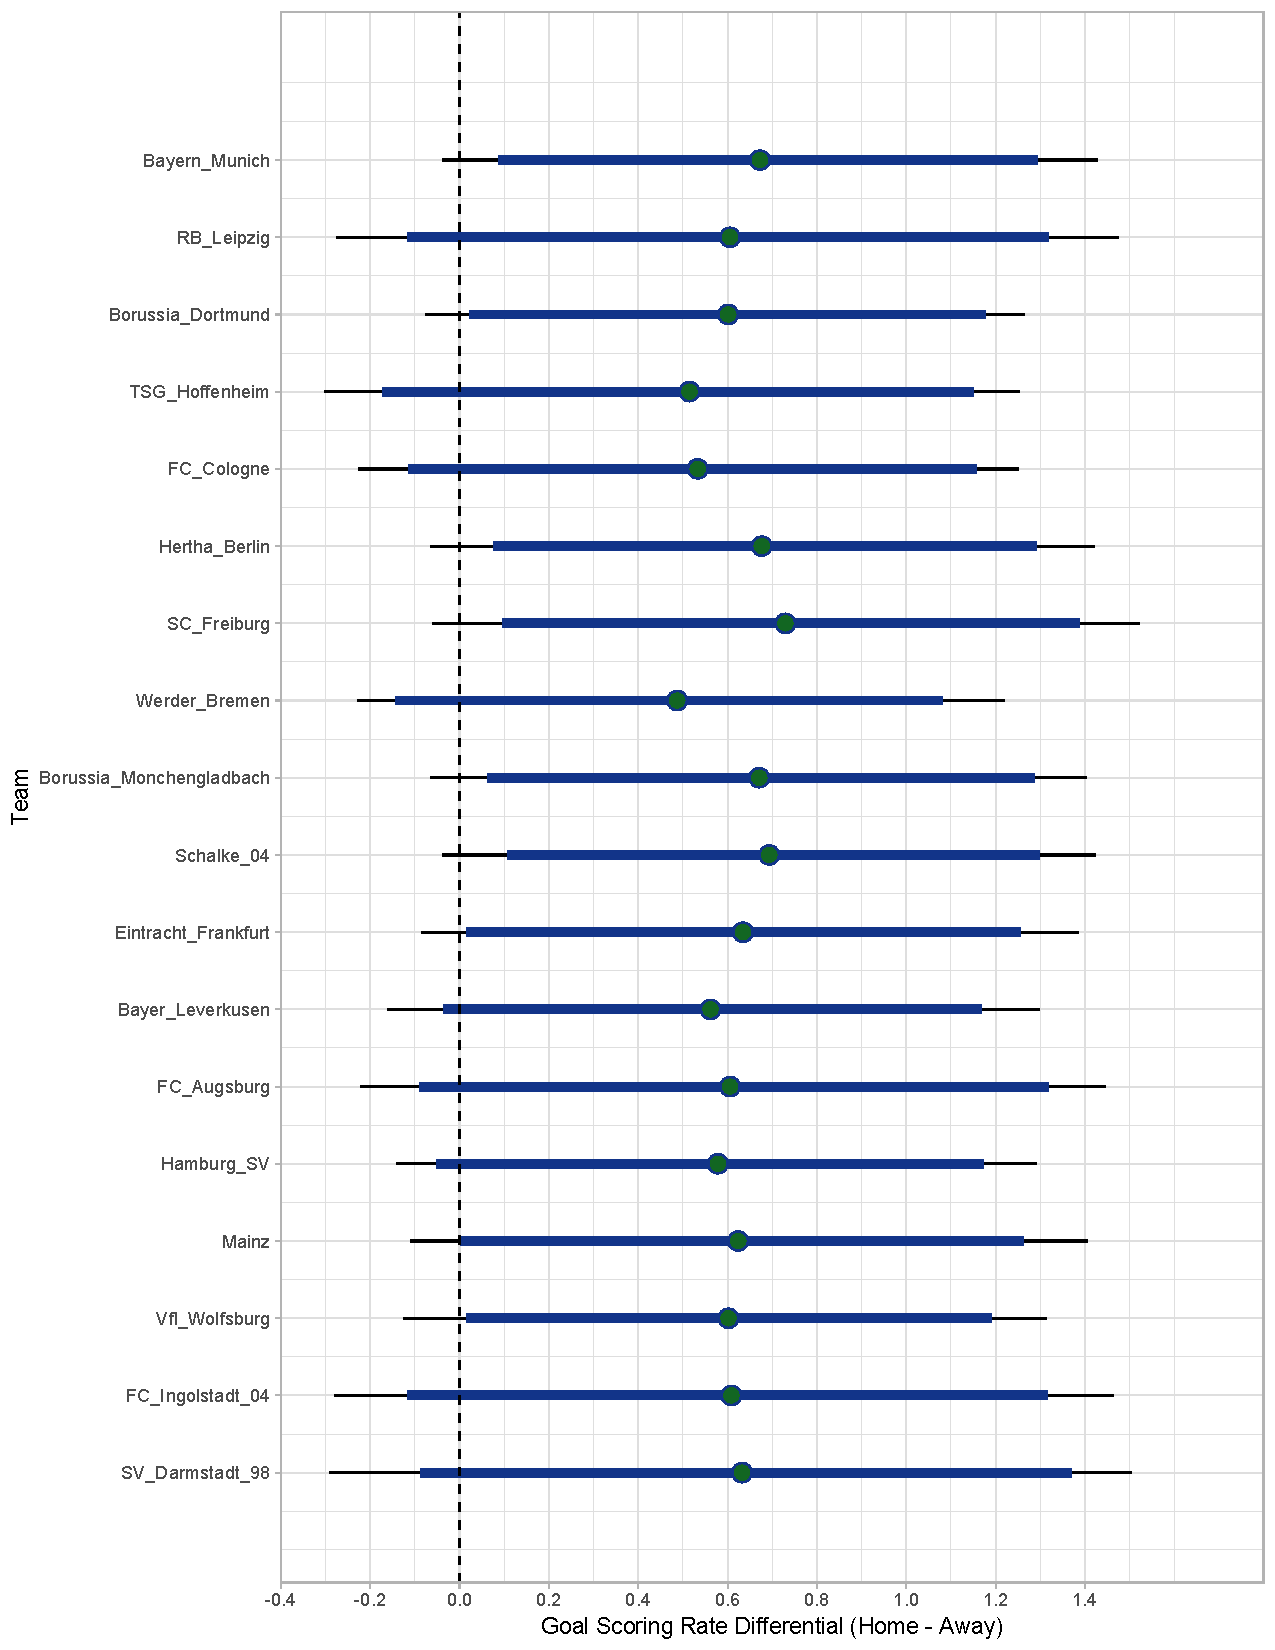
\includegraphics[width=0.90\linewidth]{HFA_Bundesliga11.pdf}}
\label{fig6}
\end{figure}

\begin{figure}
\caption{Home Field Advantage Posterior Plot for English Premier League Teams}
{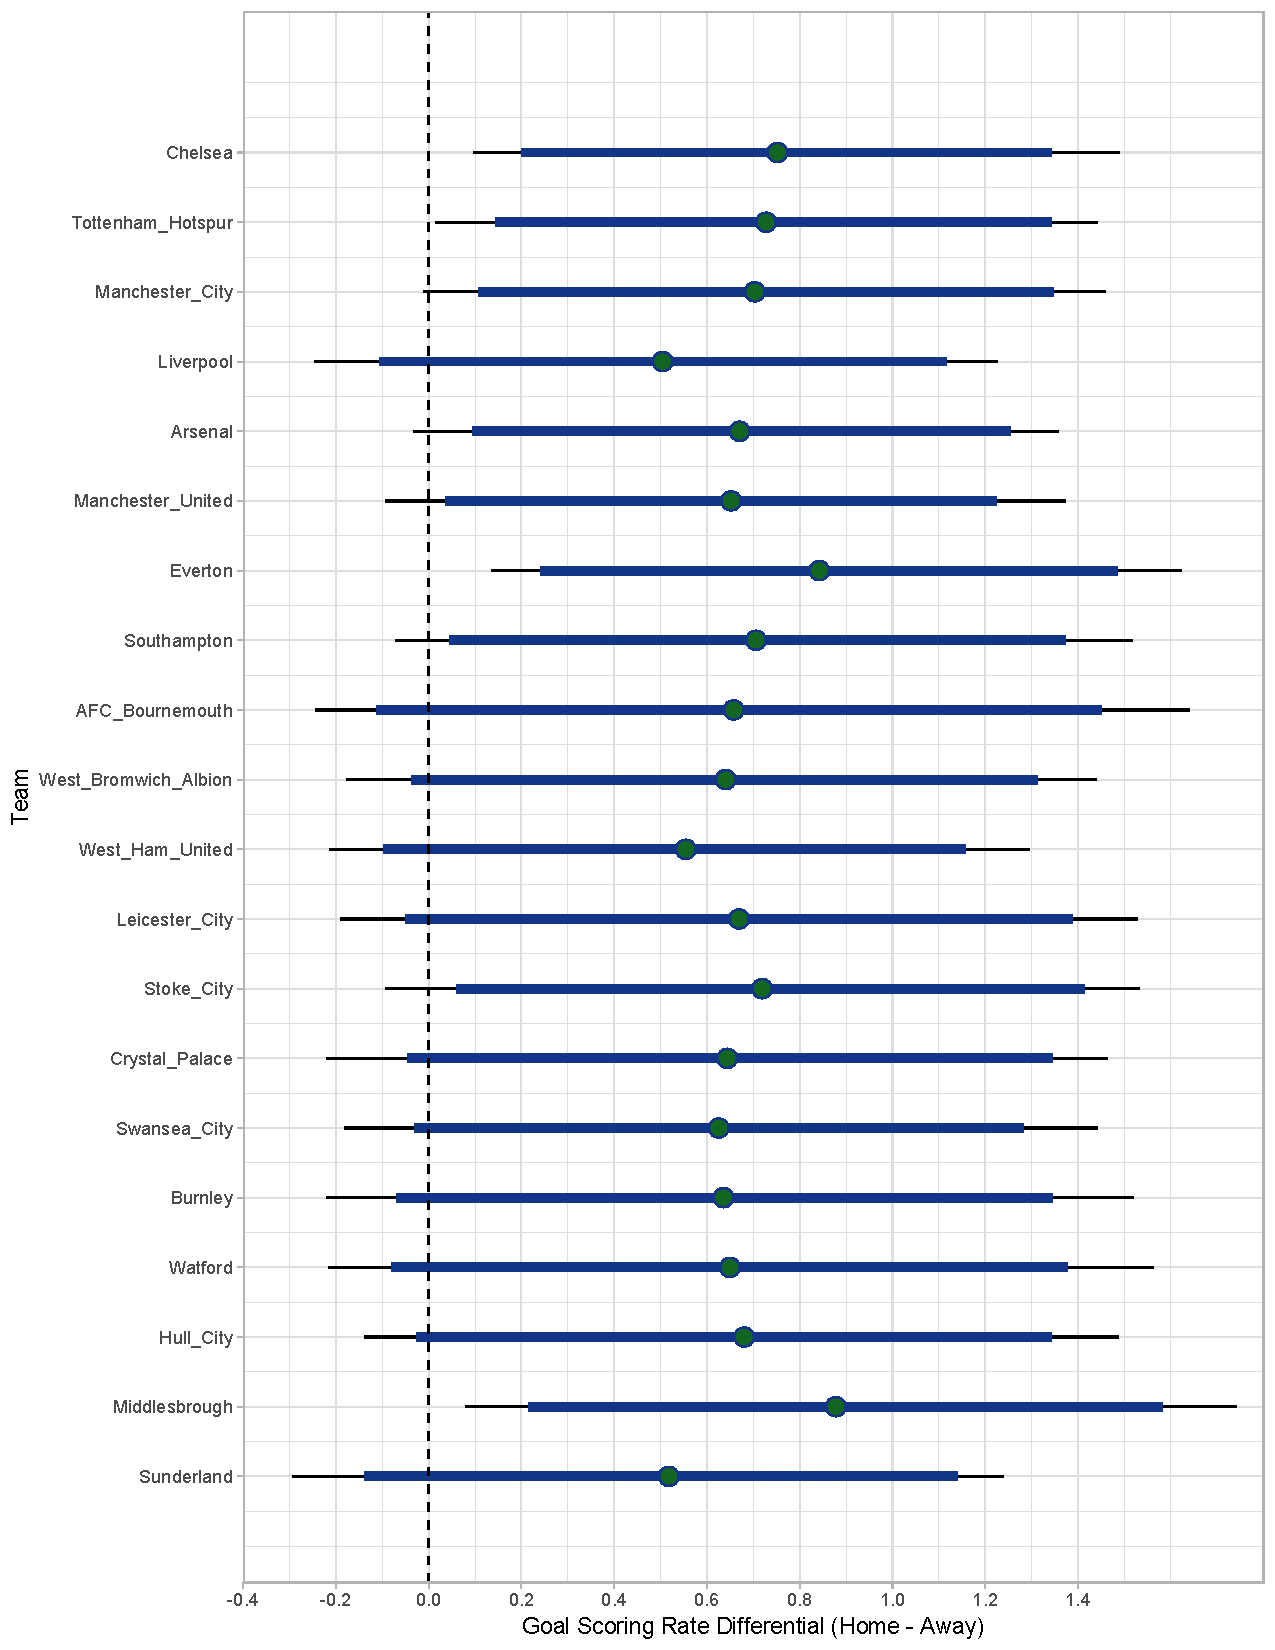
\includegraphics[width=0.90\linewidth]{HFA_EPL11.pdf}}
\label{fig7}
\end{figure}

Compared to the rest of Top 5 leagues, the English Premiere League, in Figure \ref{fig7}, shines with 4 out of 20 teams enjoy strong HFA and another 5 teams bear signs of marginal HFA. Again, we witness one bottom team enjoys the strongest HFA among all Top 5 clubs. Altogether, we observe with confidence that no team endures home field disadvantage with its corresponding uncertainty intervals lying completely to the right of the neutral line.

As part of the Stan model \citep{team2015stan}, we sample replicated data for the best scoring differential - ydiff - in the \textit{generated quantities} block. We can then check whether the actual score differences are consistent with the distribution of replicated data. For each of the 1122 seasons, we compute the 95\% and 50\% uncertainty intervals (UI) based on the replicated results. We observe that all of the actual ydiffs are in the 95\% UIs and 84.1\% in the 50\% UIs.   

As the last step of model checking, we adopt a one sport-level common parameter for all leagues and teams. After fitting the uni-parameter model to the data, we notice a 3\%  drop in the 50\%-UI containment rate from 84.1\% to 81\%.
In addition, we eliminate the middle layer of leagues from the original model and test the simplified two-layer sport-team model. The reduced model complexity is actually compensated by a minor 0.5\% increase in 50\%-UI containment rate.  
The relatively small incremental effects of team-level parametrization seem to confirm our earlier observation that only a few teams were able to show statistically strong HFA and leagues show no palpable impact on HFA distribution.



\section{Discussion}

With the unique hierarchical view and modeling flexibility of Bayesian inferential analysis, we were able to explore the locality of sources of home field advantage. Mirroring the organization structure of professional soccer competition, we originally proposed a three-level (sport-league-team) vertical view of HFA and tested it with maximum home and away scoring data covering seasons of 2000/01 to 2016/17. Further, we tested other configurations of the multilevel model structure, namely one-level model with sport only and two-level model without the middle layer of leagues. 



Unexpectedly, we found no signs of significant HFA variation at the middle league level. 
A possible explanation to this finding is that the traveling distances within most European countries are within one time-zone, and therefore are unlikely to cause any anything other than negligible fatigue. This also highlights one major limitation of our study.  The inherent geographical proximity minimizes the effect of traveling induced by league-authored schedules.

But even more remarkedly is the revelation from the post-hoc comparative analysis of goodness of fit between the single-level model and the sport-team double-deck model. Considering the fact the single-level model already measures around 81\% in terms of predictive accuracy, we would trade off the appeal of 3\% extra improvement offered by the two-level model for the ultra-simple uni-parameter model for practical reasons. For the purpose of conducting better HFA research, we might need to reorient the research field toward a broader and more encompassing unit of analysis - sport, which dictates the rules, format, and especially on-field rulings via the referees as delegates from the governing bodies.



We all know that the home filed advantage exists in all sports with varying degrees. A great deal of future research efforts should be devoted to the inter-sport investigation of HFA and quantifying the subjectivity of refereeing standards. 
Refereeing controversies regularly arise in professional competitions. Barcelona coach Ernesto Valverde complained on March 1, 2018 about an “invisible penalty” awarded to Las Palmas during the match that ended  in 1-1 draw.
The Spanish Football Federation (RFEF) has announced it is seeking approval from the International Football Association Board (IFAB) to roll out VAR ( video assistant referee)  in La Liga at the start of the 2018-19 season. VAR is already active in the top divisions in both Italy and Germany, while in England it has been tested on a trial basis in the current 2017/18 season in selected domestic cup games. It might be just pure coincidence that Serie A and Bundesliga showed the least extent of HFA in our analysis, given the role of VAR. 

Systems like VAR in soccer are purported to correct clear and obvious refereeing errors, regarding decisions on goals, red cards, penalties and cases of mistaken identity. If implementation of such machine-assisted officiating  systems becomes widespread, we can expect a clear downward trend with regard to the effect size of home field advantage. When enough machine-generated officiating data are available, we should incorporate the technology related factors into our models accordingly and assess their contributions to our understanding of HFA at the sport level. Winning on home turf and picking up points away has long been cited as the path to success in soccer. We would argue that the same mentality is driving home field advantage, as long as the enthusiastic fans are in the stands and voicing out their enthusiasms to the right target - the referees supposedly.   
 

\newpage
\begin{acknowledgement}

We would like to thank ESPN FC for compiling the season-level club performance data and allow public access.

\end{acknowledgement}

\newpage

%\bibliographystyle{name}
\bibliography{Soccer,Bayesian}
\end{document}
